\documentclass[12pt]{article}
\usepackage[utf8]{inputenc}
\usepackage{csquotes, amsmath, amssymb, graphicx, geometry, multicol}
\geometry{margin=1in}

\setlength{\parindent}{0in}

\begin{document}

\begin{titlepage}

\begin{center}
    \Huge{Properties of figures}
    
    \vspace{1in}
    
    \Large{Simon Wu}
    
    \Large{March 5, 2021}
    
    \vspace{1in}
    
    \Large{MPM2DE-B}

    
\end{center}

\tableofcontents

\end{titlepage}

\section{Problem statement}

\begin{displayquote}

Consider a line segment $AB$ where $A(5, -7)$ and the midpoint of $AB$ is $M(-5, -1)$. If line $L_1$ passes through $B$ and is perpendicular to $AB$, and line $L_2$ is given by $y = \frac{1}{3}x + 18$, determine the equation of the circle centered at the origin that passes through the point of intersection of the lines $L_1$ and $L_2$.

\end{displayquote}

\section{Graphical solution}

\begin{figure}[h]
\caption{A GeoGebra model of the situation.}
%\centering
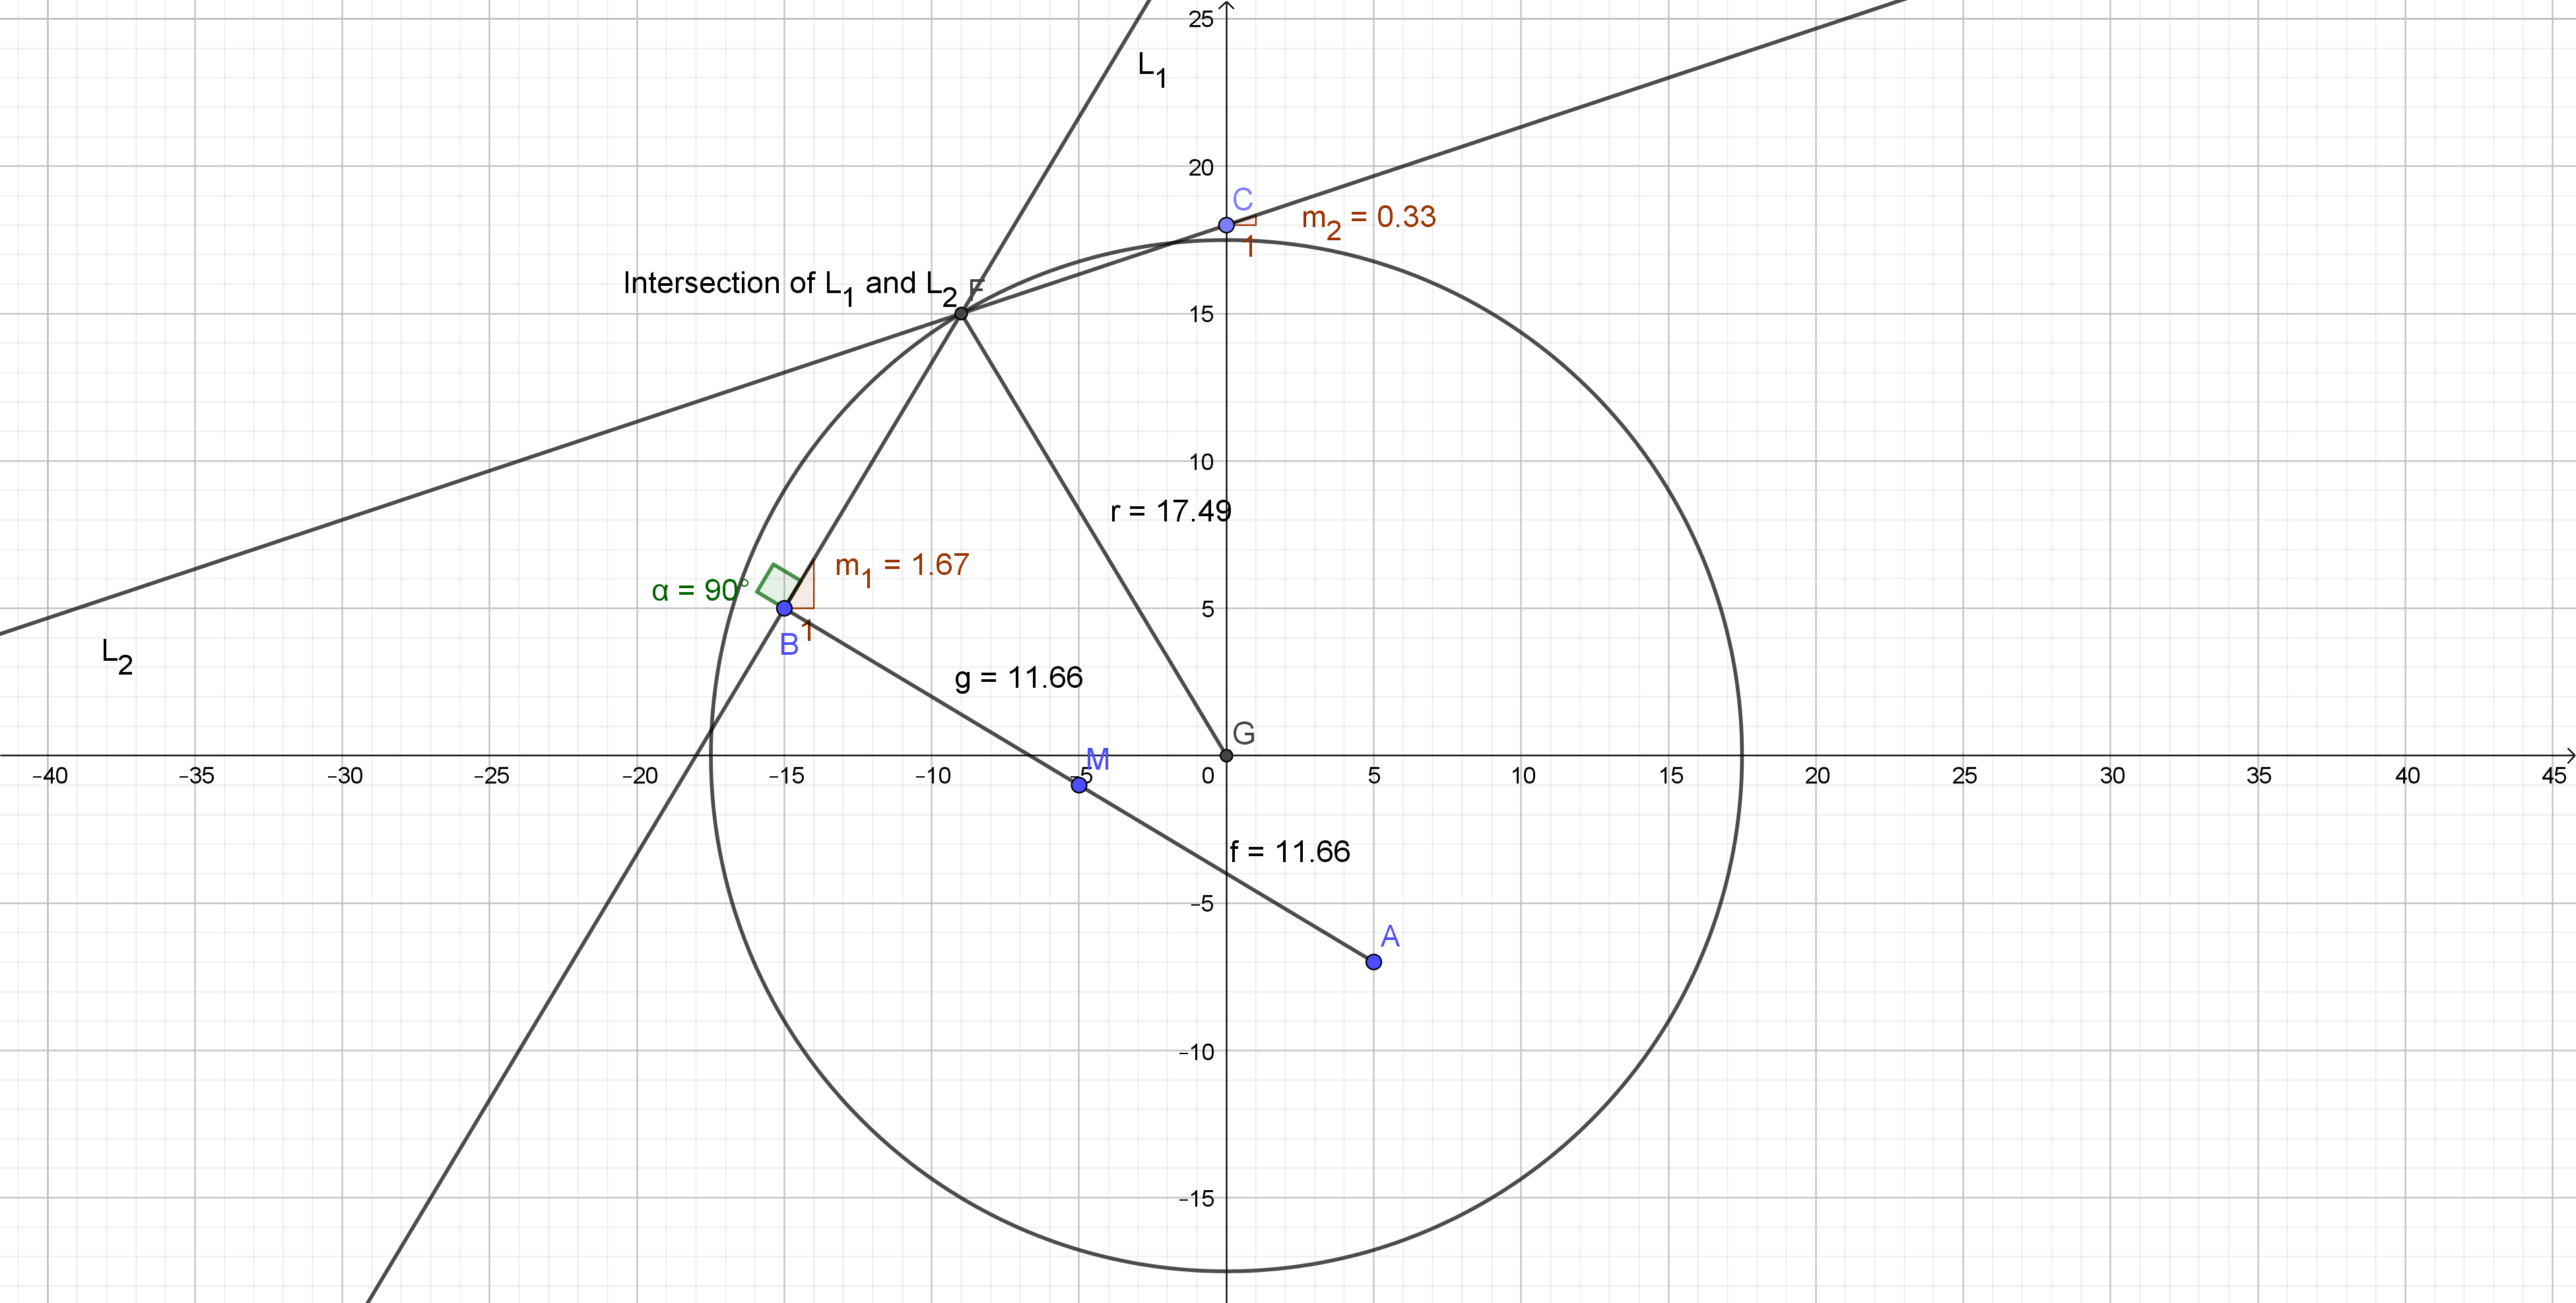
\includegraphics[width=6.5in]{circle2}
\label{fig:geogebra}
\end{figure}

As can be seen in Figure \ref{fig:geogebra}, the desired circle is centered at the origin and has a radius $r=17.49$. The equation of the circle is therefore given by:

\begin{align*}
x^2 + y^2 &= r^2\\
x^2 + y^2 &=305.90\text{ }\blacksquare
\end{align*}

\newpage

\section{Algebraic solution}

\subsection{Determining $B$}

Let the point $B$ be defined as $B(x_B, y_B)$. $M$ is the midpoint of $AB$, therefore, by the midpoint formula:

\begin{equation}
\begin{split}
\left(\frac{x_A + x_B}{2}, \frac{y_A+y_B}{2}\right) &= (x_M, y_M)\\
\left(\frac{5 + x_B}{2}, \frac{-7+y_B}{2}\right) &= (-5, -1)
\end{split}
\end{equation}

\begin{multicols}{2}

Solving for $x_B$:

\begin{equation}
\begin{split}
\frac{5+x_B}{2} &= -5\\
5 + x_B &= -10\\
x_B &= -15
\end{split}
\end{equation}

\columnbreak

Solving for $y_B$:

\begin{equation}
\begin{split}
\frac{-7+y_B}{2} &= -1\\
-7 + y_B &= -2\\
y_B &= 5
\end{split}
\end{equation}

\end{multicols}

From equations $(1)$, $(2)$ and $(3)$, we have determined the point $B(-15,5)$.

\subsection{Determining the slope of $L_1$}

The slope $m_{AB}$ of $AB$ is given by:

\begin{equation}
\begin{split}
m_{AB} &= \frac{y_B - y_A}{x_B - x_A}
\end{split}
\end{equation}

$L_1$ is perpendicular to $AB$, so its slope $m_1$ must be the negative reciprocal of $m_{AB}$.

\begin{equation}
\begin{split}
m_{1} &= -\frac{1}{m_{AB}}\\
m_{1}&= \frac{x_B - x_A}{y_B - y_A}\\
m_{1}&= -\frac{-15 -5}{5 - (-7)}\\
m_{1}&= -\frac{-20}{12}\\
m_{1}&= \frac{5}{3}
\end{split}
\end{equation}

\newpage

\subsection{Determining the equation of $L_1$}

We have determined the slope of $L_1$ and a point that $L_1$ passes through from $(2)$, $(3)$ and $(5)$, so we can now determine an equation for $L_1$.

\begin{equation}\begin{split}
y &= mx + b\\
y_B &= m_1\cdot x_B + b\\
b &= y_B - m_1\cdot x_B\\
b &= 5 - \frac{5}{3}(-15)\\
b &= 5 + 25\\
b &= 30
\end{split}\end{equation}

The equation for $L_1$ is given by:

\begin{equation}\begin{split}
y = \frac{5}{3}x + 30
\end{split}\end{equation}

\subsection{Finding the point of intersection of $L_1$ and $L_2$}

Now that the equations for both $L_1$ and $L_2$ are known, we have a system of linear equations that can be solved to determine the point of intersection $P(x_I, y_I)$ of the two lines.

\begin{equation}
\begin{cases}
y_I = \frac{5}{3}x_I + 30\\
y_I = \frac{1}{3}x_I + 18
\end{cases}
\end{equation}

This is a very simple system to solve, because both equations have $y$ isolated already. We can therefore just substitute.

\begin{equation}\begin{split}
\frac{5}{3}x_I + 30 &= \frac{1}{3}x_I + 18\\
\frac{4}{3}x_I &= -12\\
x_I &= -12\cdot\left(\frac{3}{4}\right)\\
x_I &= -9
\end{split}\end{equation}

We can substitute this value of $X_I$ back into one of the equations to determine $y_I$.

\begin{equation}\begin{split}
y_I = \frac{1}{3}\cdot (-9) + 18 = 15
\end{split}\end{equation}

The point of intersection of the lines $L_1$ and $L_2$ is $(x_I, y_I)=(-9, 15)$.

\newpage

\subsection{Determining the equation of the circle}

The circle is centered at the origin $O(0,0)$, so the equation of the circle will take the form of $x^2 + y^2 = r^2$, where $r$ is the radius of the circle.

Knowing that the point of intersection of $L_1$ and $L_2$, $P(x_I, y_I)=(-9, 15)$, is passed through by the circle, the coordinates $(-9, 15)$ must satisfy the equation of the circle, and we can solve for the unknown value of $r_2$ in this way.

\begin{equation}\begin{split}
x^2 + y^2 &= r^2\\
x_I^2 + y_I^2 &= r^2\\
(-9)^2 + 15^2 &= r^2\\
81 + 225 &= r^2\\
r^2 &= 306
\end{split}\end{equation}

The equation of the circle is therefore:

\begin{equation}\begin{split}
x^2 + y^2 &= 306\text{ }\blacksquare
\end{split}\end{equation}

This is corroborated by my graphical solution in GeoGebra from Figure \ref{fig:geogebra}: there is an error of only $0.1$ in the graphical solution, which is reasonable, due to the accuracy of numbers that GeoGebra displays.

\end{document}
